\begin{abox}
	Assignment-S01\\
	\vspace{0.5cm}
	 Coulomb's Law, Gauss Law and Electrostatic Potential
	\end{abox}
\begin{enumerate}
	\item $\left. \right. $
	\begin{answer}$\left. \right. $
		\begin{figure}[H]
			\centering
			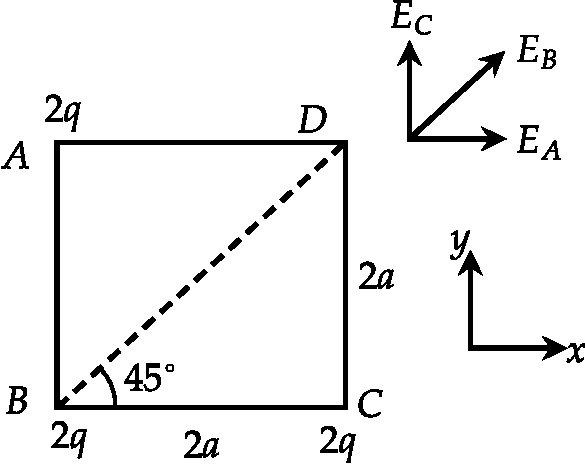
\includegraphics[height=4cm,width=5cm]{Assi-S01}
		\end{figure}
		\begin{align*}
		\text{ Electric field}&\text{ due to charge at A,}\\
		E_{A}&=\frac{2 q}{4 \pi \varepsilon_{0}(2 a)^{2}} \text { along } \mathrm{AD}\\
	\text{	Electric field }&\text{due to charge at $\mathrm{C}$,}\\
		E_{C}&=E_{A}=\frac{2 q}{4 \pi \varepsilon_{0}(2 a)^{2}} \text { along } \mathrm{CD}\\
		\text{Electric field}&\text{ due to charge at D,}\\
		E_{B}&=\frac{2 q}{4 \pi \varepsilon_{0}(2 \sqrt{2} a)^{2}} \text { along BD }\\
	\text{	Resultant along $x$-direction is }E_{x}&=E_{A}+E_{B} \cos 45=E_{A}+\frac{E_{B}}{\sqrt{2}}\\
	\text{	Resultant along $x$-direction is }E_{y}&=E_{C}+E_{B} \cos 45=E_{A}+\frac{E_{B}}{\sqrt{2}}=E_{x}\\
		\text{Thus magnitude of resultant field is }E&=\sqrt{E_{x}^{2}+E_{y}^{2}}=\sqrt{2} E_{x}=\sqrt{2}\left(E_{A}+\frac{E_{B}}{\sqrt{2}}\right)=\sqrt{2} E_{A}+E_{B}\\
		E&=\sqrt{2} \frac{2 q}{4 \pi \varepsilon_{0}(2 a)^{2}}+\frac{2 q}{4 \pi \varepsilon_{0}(2 \sqrt{2} a)^{2}}\\
		E&=\frac{2 q}{4 \pi \varepsilon_{0}(2 a)^{2}}\left[\sqrt{2}+\frac{1}{2}\right]\text{ and direction along field }E_{B} .
		\end{align*}
	\end{answer}
\item $\left. \right. $
\begin{answer}$\left. \right. $
		\begin{figure}[H]
		\centering
		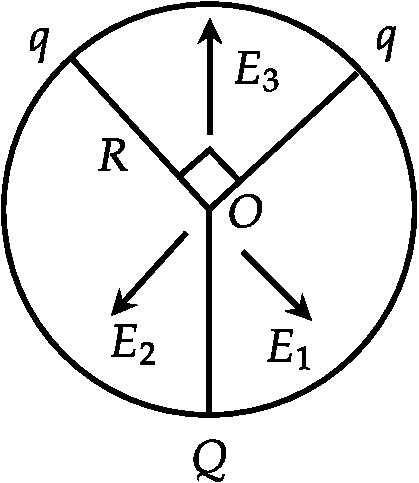
\includegraphics[height=3.3cm,width=3cm]{Assi-S02}
	\end{figure}
	\begin{align*}
	\text{(a) If }Q=q;\\
	E_{1}&=E_{2}=\frac{1}{4 \pi \varepsilon_{0}} \frac{q}{R^{2}}\text{ and }E_{3}=\frac{1}{4 \pi \varepsilon_{0}} \frac{q}{R^{2}}\text{ (upward)}\\
	\text{Resultant of $E_{1}$ and $E_{2}$ is }E_{12}&=\sqrt{E_{1}^{2}+E_{2}^{2}}=\sqrt{2} E_{1}\text{ (downward)}\\
	\because &E_{12}>E_{3}\\
	\text{Thus resultant field is }E&=E_{12}-E_{3}=\frac{1}{4 \pi \varepsilon_{0}} \frac{q}{R^{2}}(\sqrt{2}-1)\text{ in downward direction.}\\
	\text{(a) If }Q&=2 q;\\
	E_{1}=E_{2}&=\frac{1}{4 \pi \varepsilon_{0}} \frac{q}{R^{2}}\text{and}
	E_{3}=\frac{1}{4 \pi \varepsilon_{0}} \frac{2 q}{R^{2}}\text{ (upward)}\\
	\text{Resultant of $E_{1}$ and $E_{2}$ is }E_{12}&=\sqrt{E_{1}^{2}+E_{2}^{2}}=\sqrt{2} E_{1}\text{ (downward)}\\
	\because &E_{12}<E_{3}\\
	\text{Thus resultant field is }E&=E_{3}-E_{12}=\frac{1}{4 \pi \varepsilon_{0}} \frac{q}{R^{2}}(2-\sqrt{2})\text{ in upward direction.}
	\end{align*}
\end{answer}
\item $\left. \right. $
\begin{answer}$\left. \right. $
		\begin{figure}[H]
		\centering
		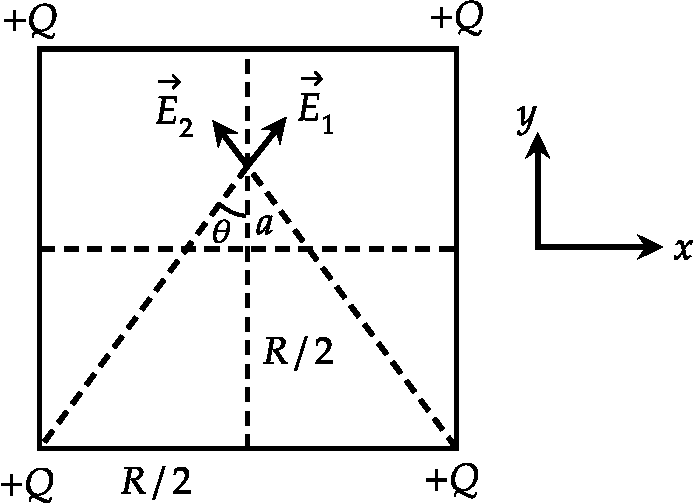
\includegraphics[height=4.5cm,width=6cm]{Assi-S03}
	\end{figure}
	\begin{figure}[H]
	\centering
	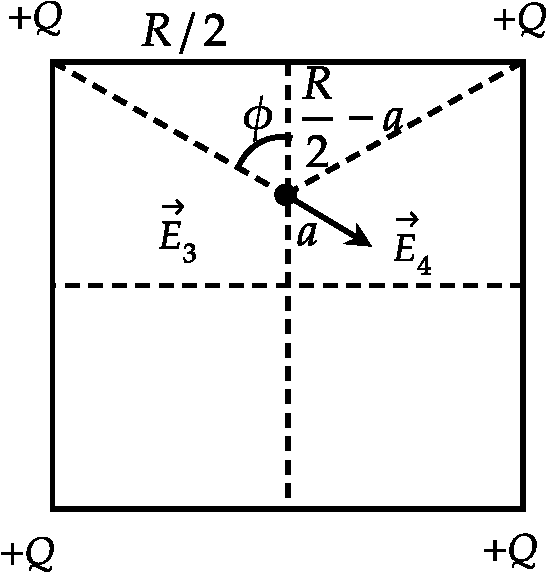
\includegraphics[height=4.5cm,width=4.3cm]{Assi-S04}
\end{figure}
	\begin{align*}
	E_{1}&=E_{2}=\frac{k Q}{\left[\left(a+\frac{R}{2}\right)^{2}+\frac{R^{2}}{4}\right]^{3 / 2}} \approx \frac{k Q}{\left[\frac{R^{2}}{2}\right]^{\frac{3}{2}}} \quad \because a<<R / 2\\ \text{Resultant field }E_{12, y}&=2 E_{1} \cos \theta\\
	E_{12, y} \approx \frac{2 k Q}{\left[\frac{R^{2}}{2}\right]^{\frac{3}{2}}}\left(a+\frac{R}{2}\right)&=\frac{4 \sqrt{2} k Q}{R^{3}}\left(a+\frac{R}{2}\right) \\
	\text { Similarly; } E_{3}&=E_{4}=\frac{k Q}{\left[\left(\frac{R}{2}-a\right)^{2}+\frac{R^{2}}{4}\right]^{3 / 2}} \approx \frac{k Q}{\left[\frac{R^{2}}{2}\right]^{\frac{3}{2}}} \\
	\text { Resultant } E_{34, y}&=2 E_{3} \cos \phi \approx \frac{2 k Q}{\left[\frac{R^{2}}{2}\right]^{\frac{3}{2}}}\left(\frac{R}{2}-a\right) \\
	\Rightarrow E_{34, y}&=\frac{4 \sqrt{2} k Q}{R^{3}}\left(\frac{R}{2}-a\right) \\
	\text { Resultant } E&=\frac{4 \sqrt{2} k Q}{R^{3}}\left[\left(\frac{R}{2}-a\right)-\left(\frac{R}{2}+a\right)\right]=-\frac{8 \sqrt{2} k Q}{R^{3}} a\\
\Rightarrow E&=\frac{-\sqrt{2}}{R^{3}} \times \frac{1}{4 \pi \varepsilon_{0}} Q a \Rightarrow E=-\frac{2 \sqrt{2} Q}{\pi \varepsilon_{0} R^{3}} a\\
	\Rightarrow F&=Q E=-\frac{2 \sqrt{2} Q^{2}}{\pi \varepsilon_{0} R^{3}} a=-\alpha a \Rightarrow \omega=\sqrt{\frac{\alpha}{m}}=\sqrt{\frac{2 \sqrt{2} Q^{2}}{\pi \varepsilon_{0} m R^{3}}}
	\end{align*}
\end{answer}
\item $\left. \right. $
\begin{answer}
	\begin{align*}
 \text{(a) }\vec{E}&=\frac{\lambda}{2 \pi \varepsilon_{0} r} \hat{r}=\frac{\lambda}{2 \pi \varepsilon_{0} r^{2}} \vec{r}=\frac{\lambda}{2 \pi \varepsilon_{0}\left(a^{2}+b^{2}\right)}(a \hat{x}+b \hat{y}) \quad \because r=\sqrt{a^{2}+b^{2}}\\
	\text{(b) }\vec{E}&=\frac{\lambda}{2 \pi \varepsilon_{0} r} \hat{r}=\frac{\lambda}{2 \pi \varepsilon_{0} \sqrt{x^{2}+y^{2}}} \hat{r}=\frac{2 \times 9 \times 10^{9} \times 10 \times 10^{-9}}{\sqrt{6^{2}+8^{2}}}=18 \hat{r} V / m
	\end{align*}
\end{answer}
\item $\left. \right. $
\begin{answer}
	\begin{align*}
\text{(a) }E&=\frac{1}{4 \pi \varepsilon_{0}} \frac{Q x}{\left(R^{2}+x^{2}\right)^{3 / 2}}\\
\text{	For maximum }E, \frac{d E}{d x}&=0 \Rightarrow \frac{Q}{4 \pi \varepsilon_{0}}\left[\frac{\left(R^{2}+x^{2}\right)^{3 / 2}-x \times 3 / 2 \sqrt{R^{2}+x^{2}} \times 2 x}{\left(R^{2}+x^{2}\right)^{3}}\right]=0\\ \Rightarrow\left(R^{2}+x^{2}\right)^{3 / 2}&=3 x^{2} \sqrt{R^{2}+x^{2}} \Rightarrow R^{2}+x^{2}=3 x^{2} \Rightarrow R^{2}=2 x^{2} \Rightarrow x=\frac{R}{\sqrt{2}}\\
	\text{(b) The electric field at point $P$ is }\vec{E}&=\frac{Q x}{4 \pi \varepsilon_{0}\left(R^{2}+x^{2}\right)^{3 / 2}} \hat{x}\\
\text{	Recall the elementary equations, }V&=-\int_{\infty}^{x} \vec{E} \cdot d \vec{l} \Rightarrow V=\frac{Q}{4 \pi \varepsilon_{0} \sqrt{R^{2}+x^{2}}}.\\
	\text{(c) }\vec{E}&=\frac{Q x}{4 \pi \varepsilon_{0}\left(R^{2}+x^{2}\right)^{3 / 2}} \hat{x} \approx \frac{Q x}{4 \pi \varepsilon_{0} R^{3}} \quad \because R \gg>x\\ \vec{F}&=-q \vec{E},\text{ one gets, }-q \frac{Q x}{4 \pi \varepsilon_{0} R^{3}}=F=m \ddot{x}\\
	\text{Small oscillations have the same form as }&\text{simple harmonic oscillations, i.e,} \\
	\ddot{x}&=-\omega^{2} x.\text{ The angular frequency is }\omega=\sqrt{q \frac{Q}{4 \pi \varepsilon_{0} R^{3} m}}.
	\end{align*}
\end{answer}
\item $\left. \right. $
\begin{answer}$\left. \right. $
		\begin{figure}[H]
		\centering
		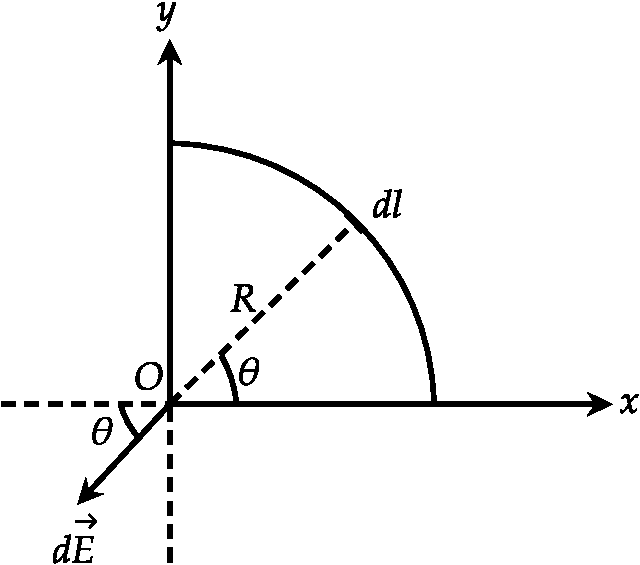
\includegraphics[height=4cm,width=4.5cm]{Assi-S05}
	\end{figure}
	\begin{align*}
	\vec{E}&=-E_{x} \hat{x}-E_{y} \hat{y}\\
	\text{where }E_{x}&=\int_{\text {line }} d E \cos \theta, E_{y}=\int_{\text {line }} d E \sin \theta.\\
\text{	and }d E&=\frac{1}{4 \pi \varepsilon_{0}} \frac{\lambda d l}{R^{2}}.\\
	E_{x}&=\int_{\text {line }} \frac{1}{4 \pi \varepsilon_{0}} \frac{\lambda d l}{R^{2}} \cos \theta=\frac{\lambda}{4 \pi \varepsilon_{0}} \int_{0}^{\pi / 2} \cos \theta \frac{R d \theta}{R^{2}} \\
	\Rightarrow E_{x}&=\frac{\lambda}{4 \pi \varepsilon_{0} R}[\sin \theta]_{0}^{\pi / 2}=\frac{\lambda}{4 \pi \varepsilon_{0} R} \\
	\text { Similarly } E_{y}&=\int_{\text {line }} \frac{1}{4 \pi \varepsilon_{0}} \frac{\lambda d l}{R^{2}} \sin \theta=\frac{\lambda}{4 \pi \varepsilon_{0}} \int_{0}^{\pi / 2} \sin \theta \frac{R d \theta}{R^{2}} \\
	\Rightarrow E_{y}&=\frac{\lambda}{4 \pi \varepsilon_{0} R}[-\cos \theta]_{0}^{\pi / 2}=\frac{\lambda}{4 \pi \varepsilon_{0} R} \\
	\text { Thus } \vec{E}&=-E_{x} \hat{x}-E_{y} \hat{y}=\frac{\lambda}{4 \pi \varepsilon_{0} R}(-\hat{x}-\hat{y})
	\end{align*}
\end{answer}
\item $\left. \right. $
\begin{answer}$\left. \right. $
		\begin{figure}[H]
		\centering
		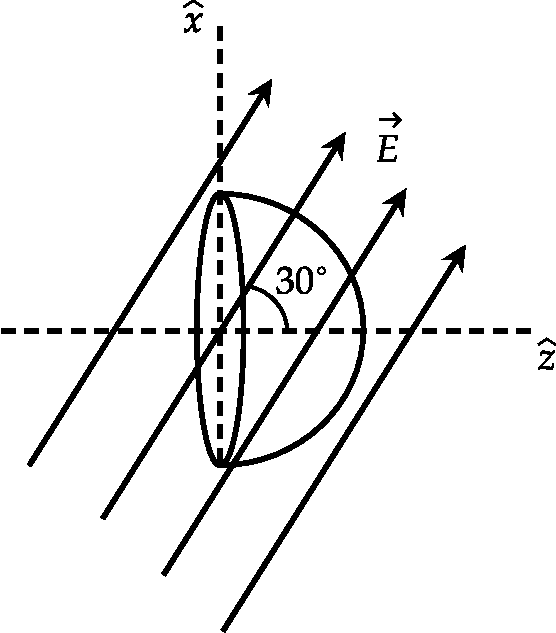
\includegraphics[height=4.5cm,width=4.5cm]{Assi-S06}
	\end{figure}
	\begin{align*}
\vec{E}&=E \cos 30 \hat{z}+E \sin 30 \hat{x}=\frac{\sqrt{3}}{2} E \hat{z}+\frac{1}{2} E \hat{x}\\
	\phi_{E}&=\int_{S} \vec{E} \cdot d \vec{a}=\iint\left(\frac{\sqrt{3}}{2} E \hat{z}+\frac{1}{2} E \hat{x}\right) \cdot\left(R^{2} \sin \theta d \theta d \phi \hat{r}\right) \\
	\phi_{E}&=R^{2} \int_{\theta=0}^{\pi / 2} \int_{\phi=0}^{2 \pi}\left(\frac{\sqrt{3}}{2} E \cos \theta+\frac{1}{2} E \sin \theta \cos \phi\right)(\sin \theta d \theta d \phi) \\
	\phi_{E}&=\frac{\sqrt{3}}{2} E R^{2} \int_{\theta=0}^{\pi / 2} \int_{\phi=0}^{2 \pi}(\cos \theta \sin \theta) d \theta d \phi+\frac{1}{2} E R^{2} \int_{\theta=0}^{\pi / 2} \int_{\phi=0}^{2 \pi}\left(\sin ^{2} \theta \cos \phi\right) d \theta d \phi \\
	\phi_{E}&=\frac{\sqrt{3}}{2} E R^{2} \times 2 \pi \times \frac{1}{2}+0=\frac{\sqrt{3}}{2} \pi R^{2} E \\
	\mathrm{OR} \\
	\phi_{E}&=\int_{S} \vec{E} \cdot d \vec{a}=E \cos 30^{0} \times \pi R^{2}=\frac{\sqrt{3}}{2} \pi R^{2} E
	\end{align*}
\end{answer}
\item $\left. \right. $
\begin{answer}$\left. \right. $
		\begin{figure}[H]
		\centering
		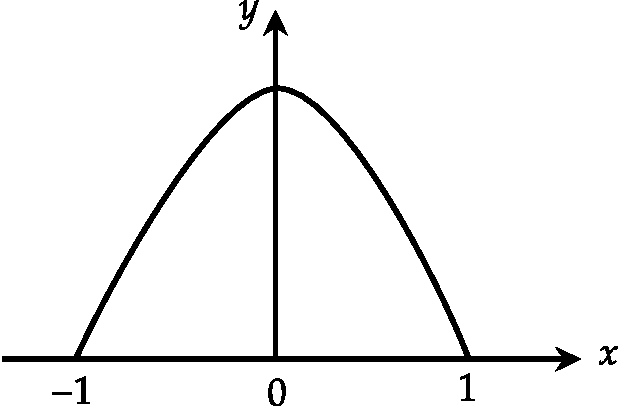
\includegraphics[height=3cm,width=4.5cm]{Assi-S07}
	\end{figure}
	Total charge on the lamina is
	\begin{align*}
	Q&=\int_{S} \sigma d a=\int_{-1}^{1} \int_{0}^{1-x^{2}} 7.5 y d x d y=\frac{7.5}{2} \int_{-1}^{1}\left(1-x^{2}\right)^{2} d x \\
	\Rightarrow Q&=\frac{7.5}{2} \int_{-1}^{1}\left(1+x^{4}-2 x^{2}\right) d x=\frac{7.5}{2}\left[x+\frac{x^{5}}{5}-2 \frac{x^{3}}{3}\right]_{-1}^{1}\\
	\Rightarrow Q&=\frac{7.5}{2}=\left[1+\frac{1}{5}-\frac{2}{3}-\left(-1-\frac{1}{5}+\frac{2}{3}\right)\right]\\&=\frac{7.5}{2}\left[1+\frac{1}{5}-\frac{2}{3}+1+\frac{1}{5}-\frac{2}{3}\right]=\frac{7.5}{2}\left[2+\frac{2}{5}-\frac{4}{3}\right]\\
	\Rightarrow Q&=\frac{7.5}{2} \times \frac{16}{15}=4 C
	\end{align*}
\end{answer}
\item $\left. \right. $
\begin{answer}
	\begin{align*}
\oint_{S} \vec{E} \cdot d \vec{a}&=\frac{1}{\varepsilon_{0}} Q_{\text {enc }} \Rightarrow|\vec{E}| \times 4 \pi r^{2}=\frac{1}{\varepsilon_{0}} \int_{0}^{r} \rho_{0}\left(1-\frac{a r}{R}\right) 4 \pi r^{2} d r\\
	\Rightarrow|\vec{E}| \times 4 \pi r^{2}&=\frac{4 \pi \rho_{0}}{\varepsilon_{0}} \int_{0}^{r}\left(r^{2}-\frac{a r^{3}}{R}\right) r^{2} d r\\&=\frac{4 \pi \rho_{0}}{\varepsilon_{0}}\left(\frac{r^{3}}{3}-\frac{a r^{4}}{4 R}\right) \Rightarrow|\vec{E}|=\frac{\rho_{0}}{\varepsilon_{0}}\left(\frac{r}{3}-\frac{a r^{2}}{4 R}\right)\\
	\text{(a) The electric field at }r&=R / 2 ; \Rightarrow|\vec{E}|=\frac{\rho_{0}}{\varepsilon_{0}}\left(\frac{R}{6}-\frac{a R^{2}}{16 R}\right)=\frac{\rho_{0} R}{2 \varepsilon_{0}}\left(\frac{1}{3}-\frac{a}{8}\right)\\
\text{	(b) The electric field at }r&=R ;|\vec{E}|=\frac{\rho_{0}}{\varepsilon_{0}}\left(\frac{R}{3}-\frac{a R^{2}}{4 R}\right)=\frac{\rho_{0} R}{\varepsilon_{0}}\left(\frac{1}{3}-\frac{a}{4}\right)\\
	\text{(c) For maximum electric field }&\frac{d E}{d r}=0.\\
	\because E&=\frac{\rho_{0}}{\varepsilon_{0}}\left(\frac{r}{3}-\frac{a r^{2}}{4 R}\right) \Rightarrow \frac{d E}{d r}=\frac{\rho_{0}}{\varepsilon_{0}}\left(\frac{1}{3}-\frac{2 a r}{4 R}\right)\\&=0 \Rightarrow \frac{2 a r}{4 R}=\frac{1}{3} \Rightarrow r=\frac{2 R}{3 a} \\
	\frac{d^{2} E}{d r^{2}}&=-\frac{\rho_{0}}{\varepsilon_{0}} \frac{2 a r}{4 R}=-v e .\\
\text{	Thus maximum value is}\\
	\because E_{\max }&=\frac{\rho_{0}}{\varepsilon_{0}}\left[\frac{1}{3} \frac{2 R}{3 a}-\frac{a}{4 R}\left(\frac{2 R}{3 a}\right)^{2}\right]\\&=\frac{\rho_{0}}{\varepsilon_{0}}\left[\frac{2 R}{9 a}-\frac{a}{4 R} \frac{4 R^{2}}{9 a^{2}}\right]=\frac{\rho_{0}}{\varepsilon_{0}}\left[\frac{2 R}{9 a}-\frac{R}{9 a}\right]=\frac{\rho_{0} R}{9 a \varepsilon_{0}}\\
	\text{(d) }\because E_{r=R / 2}&=1.25 E_{r=R} \Rightarrow \frac{\rho_{0}}{\varepsilon_{0}}\left(\frac{R / 2}{3}-\frac{a R^{2} / 4}{4 R}\right)=1.25 \frac{\rho_{0}}{\varepsilon_{0}}\left(\frac{R}{3}-\frac{a R^{2}}{4 R}\right)\\
	\Rightarrow\left(\frac{1}{6}-\frac{a}{16}\right)&=\frac{5}{4}\left(\frac{1}{3}-\frac{a}{4}\right) \Rightarrow\left(\frac{1}{6}-\frac{a}{16}\right)\\&=\left(\frac{5}{12}-\frac{5 a}{16}\right) \Rightarrow \frac{5 a}{16}-\frac{a}{16}=\frac{5}{12}-\frac{1}{6}\\
	\Rightarrow \frac{4 a}{16}&=\frac{5-2}{12} \Rightarrow \frac{a}{4}=\frac{3}{12} \Rightarrow a=1
	\end{align*}
\end{answer}
\item $\left. \right. $
\begin{answer}$\left. \right. $
		\begin{figure}[H]
		\centering
		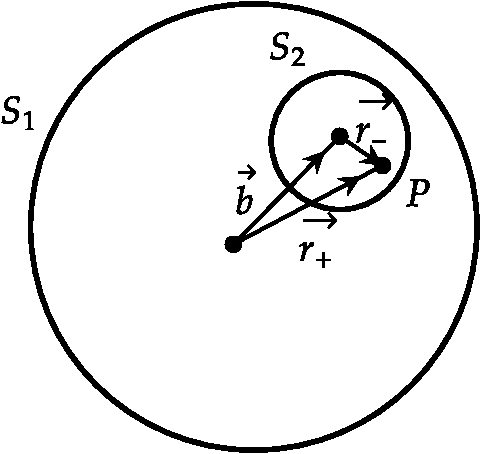
\includegraphics[height=4cm,width=4.3cm]{Assi-S08}
	\end{figure}
	\begin{align*}
	\text{ Electric field at $P$ due to $S_{1}$ is }\vec{E}_{1}&=\frac{\rho}{3 \varepsilon_{0}} \vec{r}_{+}\\
\text{	Electric field at $P$ due to $S_{2}$ (assume $-\rho$ ) is }\vec{E}_{2}&=\frac{-\rho}{3 \varepsilon_{0}} \vec{r}_{-}\\
\text{	Thus }\vec{E}=\vec{E}_{1}+\vec{E}_{2}&=\frac{\rho}{3 \varepsilon_{0}}\left(\vec{r}_{+}-\vec{r}_{-}\right) ; \\
\quad \because \vec{b}+\vec{r}_{-}=\vec{r}_{+} \Rightarrow \vec{r}_{+}-\vec{r}_{-}&=\vec{b}\\
\Rightarrow \vec{E}&=\frac{\rho}{3 \varepsilon_{0}} \vec{b}
	\end{align*}
\end{answer}
\item $\left. \right. $
\begin{answer}$\left. \right. $
		\begin{figure}[H]
		\centering
		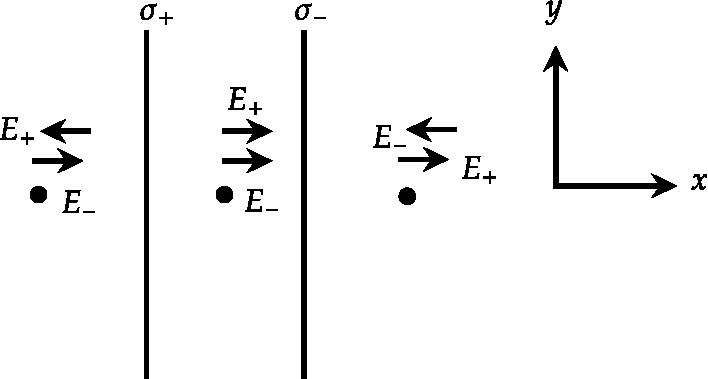
\includegraphics[height=3.5cm,width=7cm]{Assi-S09}
	\end{figure}
	(a) Electric field between the sheet is
	\begin{align*}
	|\vec{E}|&=\frac{\sigma_{+}}{2 \varepsilon_{0}}+\frac{\sigma_{-}}{2 \varepsilon_{0}}=\frac{6.8 \times 10^{-6}}{2 \varepsilon_{0}}+\frac{4.3 \times 10^{-6}}{2 \varepsilon_{0}} \\
	\Rightarrow|\vec{E}|&=\frac{11.2 \times 10^{-6}}{2 \times 8.86 \times 10^{-12}}=0.626 \times 10^{6} \mathrm{~N} / C \\
	\Rightarrow \vec{E}&=6.3 \times 10^{5} \hat{x} \mathrm{~N} / C\\
	\text{(b) Electric }&\text{field outside the sheet (towards right) is}\\
	|\vec{E}|&=\frac{\sigma_{+}}{2 \varepsilon_{0}}-\frac{\sigma_{-}}{2 \varepsilon_{0}}=\frac{6.8 \times 10^{-6}}{2 \varepsilon_{0}}-\frac{4.3 \times 10^{-6}}{2 \varepsilon_{0}}\\&=\frac{2.5 \times 10^{-6}}{2 \times 8.86 \times 10^{-12}}=0.141 \times 10^{6} \mathrm{~N} / \mathrm{C} \\
	\Rightarrow & \vec{E}=1.4 \times 10^{5} \hat{x} \mathrm{~N} / \mathrm{C}\\
	\text{Electric field }&	\text{outside the sheet (towards left) is }\vec{E}=-1.4 \times 10^{5} \hat{x} \mathrm{~N} / \mathrm{C}
	\end{align*}
\end{answer}
\item $\left. \right. $
\begin{answer}
	\begin{align*}
\text{(a) }\because V(r)&=A \frac{e^{-\lambda r}}{r} ; \quad \vec{E}=-\vec{\nabla} V\\&=-A\left[\frac{r e^{-\lambda r} \times(-\lambda)-e^{-\lambda r}}{r^{2}}\right] \hat{r}=\frac{A e^{-\lambda r}}{r^{2}}(1+\lambda r) \hat{r}\\
	\text{(b) }Q_{\text {enc }}&=\varepsilon_{0} \oint \vec{E} \cdot d \vec{a}=\varepsilon_{0} \int_{0}^{\pi} \int_{0}^{2 \pi} \frac{A e^{-\lambda r}}{r^{2}}(1+\lambda r) \hat{r} \cdot r^{2} \sin \theta d \theta d \phi \hat{r}\\&=4 \pi \varepsilon_{0} A e^{-\lambda r}(1+\lambda r)\\
	\text{Thus total charge }&\text{enclosed within a sphere of radius }r=\frac{1}{\lambda}\text{ is }\\
	Q_{c n c}&=4 \pi \varepsilon_{0} A e^{-\lambda \frac{1}{\lambda}}\left(1+\lambda \frac{1}{\lambda}\right)=\frac{8 \pi \varepsilon_{0} A}{e}
	\end{align*}
\end{answer}
\item $\left. \right. $
\begin{answer}
	\begin{align*}
\text{(a) At }r&=R, \quad Q_{\text {enc }}=\varepsilon_{0} \oint \vec{E} \cdot d \vec{a}=\alpha \varepsilon_{0} \int\left(1-e^{-R / R}\right) \frac{\hat{r}}{R^{2}} \cdot\left(R^{2} \sin \theta d \theta d \phi \hat{r}\right)\\
	Q_{e n c}&=\alpha \varepsilon_{0} \times \int_{0}^{\pi} \int_{0}^{2 \pi}\left(1-e^{-1}\right) \sin \theta d \theta d \phi \Rightarrow Q_{e n c}=4 \pi \alpha \varepsilon_{0}\left(1-\frac{1}{e}\right) \\
	\text { (b) } Q_{\text {enc }}&=\varepsilon_{0} \oint \vec{E} \cdot d \vec{a}=\varepsilon_{0} \int(\alpha \hat{r}+\beta \sin \theta \cos \phi \hat{\phi}) \cdot\left(r^{2} \sin \theta d \theta d \phi \hat{r}\right)=4 \pi \alpha \varepsilon_{0}
	\end{align*}
\end{answer}
\item $\left. \right. $
\begin{answer}
	\begin{align*}
 \text{(a) }V(x, y)&=3 x^{2}-3 y^{2} ; \quad\text{ Since }\nabla^{2} V=-\frac{\rho}{\varepsilon_{0}} \Rightarrow \rho=0.\\
	\because \vec{E}&=-\vec{\nabla} V \Rightarrow E_{x}=-6 x \Rightarrow E_{x}(0,0)=0 \\
	\Rightarrow E_{y}&=6 y \Rightarrow E_{y}(0,0)=0\\
	\text{(b) }\nabla^{2} V&=\frac{1}{r^{2}} \frac{\partial}{\partial r}\left(r^{2} \frac{\partial V}{\partial r}\right)+\frac{1}{r^{2} \sin \theta} \frac{\partial}{\partial \theta}\left(\sin \theta \frac{\partial V}{\partial \theta}\right)+\frac{1}{r^{2} \sin ^{2} \theta}\left(\frac{\partial^{2} V}{\partial \phi^{2}}\right)=0\\
	\Rightarrow \frac{1}{r^{2}} \frac{\partial}{\partial r}&\left(r^{2} \frac{\partial f}{\partial r} \cos \theta\right)+\frac{1}{r^{2} \sin \theta} \frac{\partial}{\partial \theta}(\sin \theta f \times-\sin \theta)=0 \\
	\Rightarrow &\frac{\cos \theta}{r^{2}}\left(r^{2} \frac{\partial^{2} f}{\partial^{2} r}+2 r \frac{\partial f}{\partial r}\right)-\frac{f}{r^{2} \sin \theta}(2 \sin \theta \cos \theta)\\&=0 \Rightarrow r^{2} \frac{\partial^{2} f}{\partial^{2} r}+2 r \frac{\partial f}{\partial r}-2 f(r)=0\\
\text{	(c) }\because \nabla^{2} \phi&=-\frac{\rho}{\varepsilon_{0}} \Rightarrow \rho=-\varepsilon_{0}\left(\nabla^{2} \phi\right)\\
	\nabla^{2} \phi&=\frac{1}{r^{2}} \frac{\partial}{\partial r}\left(r^{2} \frac{\partial \phi}{\partial r}\right)=\frac{1}{r^{2}} \frac{\partial}{\partial r}\left(r^{2} \times-\frac{\phi_{0}}{r_{0}} e^{-r / r_{0}}\right)\\&=-\frac{1}{r^{2}} \frac{\phi_{0}}{r_{0}} \frac{\partial}{\partial r}\left(r^{2} \times e^{-r / r_{0}}\right)=-\frac{1}{r^{2}} \frac{\phi_{0}}{r_{0}}\left[r^{2} \times-\frac{1}{r_{0}} e^{-r / r_{0}}+2 r e^{-r / r_{0}}\right] \\
	\Rightarrow \nabla^{2} \phi&=-\frac{\phi_{0}}{r_{0}}\left[-\frac{1}{r_{0}} e^{-r / r_{0}}+\frac{2}{r} e^{-r / \sigma_{0}}\right]\\
	\text{At a distance }r&=r_{0},\\
	\nabla^{2} \phi&=-\frac{\phi_{0}}{r_{0}}\left[\frac{1}{r_{0}} e^{-1}+\frac{2}{r_{0}} e^{-1}\right]=-\frac{\phi_{0}}{r_{0}^{2} e} \Rightarrow \rho=-\varepsilon_{0}\left(-\frac{\phi_{0}}{r_{0}^{2} e}\right)=\frac{\phi_{0} \varepsilon_{0}}{r_{0}^{2} e}
	\end{align*}
\end{answer}
\item $\left. \right. $
\begin{answer}
	 (a) The Laplace's equation in Cartesian coordinates system is
	\begin{align*}
	\nabla^{2} V=\frac{\partial^{2} V}{\partial x^{2}}=\frac{\partial^{2} V}{\partial y^{2}}+\frac{\partial^{2} V}{\partial z^{2}}=-\frac{\rho}{\varepsilon_{0}}	\end{align*}
		as $V$ is only function of $x$, we have the differential equation, $\frac{d^{2} V}{d x^{2}}=-\frac{\rho}{\varepsilon_{0}}$ by integrating we have the solution of this equation as\\
	$\frac{d V}{d x}=-\frac{\rho}{\varepsilon_{0}} x+A \Rightarrow V(x)=-\frac{\rho}{2 \varepsilon_{0}} x^{2}+A x+B \quad$ where $A$ and $B$ are constants.
	The two equations need to be solved for the following boundary conditions:
	\begin{align*}
\text{	(i) }x&=0 ; V=0\hspace{2cm}
	\text{(ii) }x=2 a ; V=V_{0}
	\end{align*}
	Substituting these boundary conditions, we get
	\begin{align*}
	\text{At }x&=0, V(0)=0=0+0+B \Rightarrow B=0\\
\text{	At }x&=2 a,\\
	V(L)&=V_{0}=-\frac{\rho}{2 \varepsilon_{0}}(2 a)^{2}+A(2 a) \Rightarrow A=\frac{V_{0}}{2 a}+\frac{\rho a}{\varepsilon_{0}} \Rightarrow V(x)=-\frac{\rho}{2 \varepsilon_{0}} x^{2}+\left(\frac{V_{0}}{2 a}+\frac{\rho a}{\varepsilon_{0}}\right) x\\
	\text{(b) }\because V(x)&=-\frac{\rho}{2 \varepsilon_{0}} x^{2}+\left(\frac{V_{0}}{2 a}+\frac{\rho a}{\varepsilon_{0}}\right) x \Rightarrow \vec{E}(x)=-\vec{\nabla} V=\left[\frac{\rho}{\varepsilon_{0}} x-\left(\frac{V_{0}}{2 a}+\frac{\rho a}{\varepsilon_{0}}\right)\right] \hat{x}
	\end{align*}
\end{answer}
\item $\left. \right. $
\begin{answer}
	\begin{align*}
	\because \nabla^{2} V&=0\\
	\text{In Cylindrical coordinate system, }\frac{1}{r} \frac{\partial}{\partial r}\left(r \frac{\partial V}{\partial r}\right)&=0 \Rightarrow V=A \ln r+B\\
	\text{Thus }10&=A \ln 2+B\text{ and }0=A \ln 5+B\\
	\Rightarrow 10&=A \ln 2-A \ln 5 \Rightarrow A=-\frac{10}{\ln (5 / 2)}\text{ and}\\ \Rightarrow B&=\frac{10 \ln 5}{\ln (5 / 2)}\\
	\Rightarrow V(r=3.5)&=A \ln 3.5+B=3.8 V
	\end{align*}
\end{answer}
\end{enumerate}